%  SingleXB
%  Created by Dave Williams on 2009-06-25.
%  

% header (fold)
\documentclass[]{article}

\usepackage{setspace, float, fancyhdr}
\usepackage[pdftex]{graphicx}
\usepackage[utf8]{inputenc}
\usepackage[round,numbers,sort&compress]{natbib} 
\addtolength{\parskip}{\baselineskip}
\setlength{\parindent}{0in}

% Multi-part figures
%\usepackage{subfigure}
% Package for including code in the document
%\usepackage{listings}

\title{A multidimensional actomyosin crossbridge model simulates radial forces and the effects of changes in sarcomere lattice spacing} 
\author{C.D.\ Williams, M.\ Regnier, T.L.\ Daniel}
\date{2009--06--25}
% header (end)

\begin{document}

\maketitle{}

\begin{abstract} 
Existing spatially explicit models of muscle contraction treat myosin as a single spring oriented parallel to the direction of contraction.
Here we describe a model of myosin, based on protein structure, that forms a four spring crossbridge (4sXB) and closely replicates the force-generating powerstroke.
This 4sXB model takes most parameters from experimental measurements and permits monitoring of phenomena not possible with a single-spring crossbridge.
The 4sXB generates radial force (orthogonal to the direction of contraction) during its power stroke similar to what physical crossbridges produce.
Also, as with physical crossbridges, the 4sXB's kinetics and force production vary with lattice spacing as angles of attachment, crossbridge geometry and diffusion distances change.
Additionally, we describe a simpler two spring crossbridge (2sXB) that replicates most qualities of the 4sXB.
Unlike the 4sXB, the length and angle of the springs comprising the 2sXB can be determined analytically for any chosen head position without the use of iterative techniques.
The forces generated by the 4sXB and the 2sXB are similar.
The rate at which the multi-spring crossbridges bind and generate force depend on lattice spacing, decreasing as lattice spacing grows. 
The axial and radial forces generated by multi-spring crossbridges increase in magnitude as lattice spacing is offset from the myosin head resting position. 
These factors are possible regulators of force production as length and lattice spacing change in the intact muscle.
\end{abstract}

Keywords: myosin; spatially-explicit model; crossbridge kinetics

% \paragraph*{Author Summary} % (fold)
% Models of muscle contraction have long treated the molecular motor myosin as a simple spring oriented parallel to its direction of movement. 
% This does not allow for the investigation of phenomena such as the perpendicular force observed during shortening, or the dependence of the maximum force produced on spacing between the contractile filaments that comprise muscle.
% We demonstrate an alternative model, computationally simple enough to use in large networked models, that incorporates both linear and torsional (angle dependent) springs. 
% This model type captures much of the behavior missing from single spring models of the crossbridge.
% paragraph author_summary (end)


\section{Introduction} %(fold)

% While individual crossbridges have been treated independently with spatial modeling, thermodynamic accounting has been introduced to the crossbridge kinetics, compliance introduced to the filaments, and multiple filaments have been arranged to mimic the lattice, the one dimensional nature of the crossbridge has continued to be used as a model of the mechanism of force generation.

Radial forces of the same order of magnitude as axial force have been shown to exist in  contracting muscles \citep{Cecchi1990, Millman1998}. 
These forces, and radial lattice spacing, have been put forward as a possible regulator of force generation \citep{Fuchs2005}. 
At the same time, increased understanding of myosin's structure has lead supported the idea that myosin generates force through the action of a lever arm \citep{Rayment1993, Uyeda1996, Huxley2000}.
Myosin's lever arm generates the strain that accompanies the powerstroke via a change in the rest angle at which the lever is attached to S1 region \citep{Huxley2000, Houdusse2001}. 
This change in angle occurs at the converter region, a flexible area that and acts as a torsional or angular spring. 
It has been suggested that these phenomena are related, i.e.\ that radial forces during crossbridge force generation are a result of lever-arm geometry \citep{Schoenberg1980b}. 

Existing theoretical and computational models of crossbridge force generation, at the filament level, have used one-dimensional crossbridges. 
As a consequence these computational studies, from the early work of \citet{Huxley1957} to more recent models \citep{Daniel1998, Chase:2004:p204, Tanner2007}, have confined themselves to forces aligned along the axes of the contractile filaments.  
From a computational standpoint, little attention has been paid to radial forces. 
Thus, the geometry of single spring crossbridge models has remained largely unchanged while the kinetics underlying transitions between force generating states have increased in complexity throughout subsequent work \citep{Pate1989, Daniel1998, Tanner2007}.
However, the lever arm mechanism of force generation by myosin suggests that inclusion of torsional springs in computational models would better reflect the underlying mechanisms of the powerstroke. 

In this paper we examine and compare two torsional spring based crossbridge models, both well suited for use in spatially explicit models of the half sarcomere. 
The first is a four spring crossbridge (4sXB) based upon the structure of the S1 and S2 regions of myosin II (Fig.~\ref{fig_xb_types}D). 
Following this, we consider a two spring crossbridge (2sXB) that replicates many of the behaviors of the 4sXB while requiring fewer computational resources (Fig.~\ref{fig_xb_types}C). 
We derive a genreralized three state kinetic system from those used by prior models \citep{Pate1989, Daniel1998, Tanner2007}. 
We quantify the radial force produced by these isolated crossbridges and how such forces increase as sarcomere lattice spacing expands.
We also investigate how changes in lattice spacing affect other properties of the isolated crossbridges, such as how optimum axial location of an available actin site for binding, the powerstroke, and detachment shifts towards the crossbridge as lattice spacing increases. 

The crossbridge models developed here, when included in spatially explicit multi-filament models of the half-sarcomere, permit investigation of the effects of radial forces and lattice spacings for the first time. 
Such models should contribute to ongoing discussions about the role that radial forces (transmitted directly or through titin) and changes in lattice spacing play in the Frank-Starling mechanism and in the regulation of Ca$^{2+}$ sensitivity \citep{Fuchs2005}. 

% % \paragraph{Comparison to previous systems} % (fold)
% This discussion owes a debt to \citet{Schoenberg1980a} and \citet{Schoenberg1980b} which contain a proposal and analysis of several different types of crossbridges, primarily two spring crossbridges where the S2 arm is represented as a linear spring and the S2-S1 junction area is represented as a torsional spring. 
% This system requires iterative solution methods, as our four spring crossbridge does, but restrains the crossbridge to an area within one S1 length of the line in which the S2 segment is set.
% % paragraph comparison_to_previous_systems (end)

% section introduction (end)


\section{Materials and Methods}  % (fold)

We consider two separate crossbridge models, the 4sXB and the 2sXB (Figs.~\ref{fig_xb_types}C-D) meant to capture a range of mechanical behaviors reported in the literature.  
These are contrasted to the traditional one-dimensional single spring model of a crossbridge (Fig.~\ref{fig_xb_types}B).

\subsection*{Geometry} % (fold)

The behavior of a crossbridge is governed by both its chemical kinetics, such as rates of binding and powerstroke, and by its geometry, the shape of the protein and the resulting physical properties.
We define geometry first since modeled crossbridge kinetics are dependent on the chosen geometry.
Spring rest angles, lengths and constants are derived from experimental measurements where available.

\paragraph{Spring configurations} % (fold)
For comparison to previous modeling results, a one-spring crossbridge (1sXB) similar to those used previously is re-implemented.
This simplest of models consists of a single linear spring parallel to the axes of the thick and thin filaments, able only to generate forces in the direction of shortening. 
This current crossbridge model implemented in most spatially-explicit computational analyses \citep{Daniel1998, Chase:2004:p204, Tanner2007} is insensitive to changes in lattice spacing, and unable to account for radial forces generated during axial shortening.

Our four-spring crossbridge (4sXB) uses two linear and two torsional springs to represent the myosin head (Fig.~\ref{fig_xb_types}D).
This allows the springs used to closely correspond to particular structures of the crossbridge.
Specifically the four springs correspond to the S2 region/rod attachment point, the S2 region, the S2 region/light chain domain (LCD) attachment point, and the LCD. 
The torsional spring at the S2/LCD attachment point mimics force generation by a lever arm via a change in the angle about the converter region \citep{Houdusse2000, Houdusse2001}. 
Since the angle at which the head attaches to actin remains unchanged in our model, the torque generated at the converter region can be accounted for in a torsional spring on the end of LCD linear spring closer to the thick filament attachment point \citep{Lauzon2001}. % TODO : Closely read Lauzon2001 
The 4sXB's use of multiple springs also allows it to calculate radial forces and other crossbridge properties that are not present in the 1sXB's one-dimensional space. 
The rest angle of the torsional spring linking the S2 domain and the LCD simulates the powerstroke by increasing during the transition from a weakly bound to a strongly bound state.
This two dimensionality allows the 4sXB to be embedded in a space that takes the distance between thick and thin filaments into account, introducing lattice spacing dependence.

The 2sXB uses one linear and one torsional spring to represent the myosin head (Fig.~\ref{fig_xb_types}C).
This crossbridge is a simplified version of the 4sXB. 
In the 2sXB movement is still generated by a lever arm, but the length of the lever arm is increased so that the distance from the thick filament to the tip of the crossbridge remains consistent with the 4sXB.
The parameters characterizing the 2sXB are chosen to match the step size, tip location and kinetics of the 2sXB to those of the 4sXB. 
The resulting 2sXB is computationally simpler than, but retains the two-dimensional nature of, the 4sXB.

Parameters for both crossbridges are derived, where possible, from existing physical measurements.
Each linear spring (one in the 1sXB, two in the 4sXB and one in the 2sXB) requires a rest length and spring constant, while each torsional spring (two in the 4sXB and one in the 2sXB) requires a rest angle and spring constant.
The lengths and angles of the springs used for the 4sXB are chosen from tomographic reconstructions of in vivo S2 lengths and x-ray crystallographic reconstructions of the S1 fragment \citep{Taylor1999, Rayment1993}.
The rest length and angle of the 2sXB are set so that the tips of the 2sXB and 4sXB are in the same location before and after the powerstroke.

% Should include a bit on spring constant derivation from Pi hydrolysis energies 
% Consider including a table of parameter values?

% paragraph spring_configurations (end)

\paragraph{Calculation of lattice spacing} % (fold)
Throughout this paper, d$_{1,0}$ spacing is derived from the geometry of the crossbridge and the lattice spacing with the least radial force. 
The model provides a measurement of spacing that is analogous to the in vivo distance between the surfaces of the thick and thin filaments.
The d$_{1,0}$ spacing is calculated from this surface-to-surface lattice spacing (ssLS) using an offset that corrects for d$_{1,0}$ being measured from the center of one thick filament to the center of another. 
Specifically, d$_{1,0}$ is given by $\rm{d}_{1,0} = 1.5 (ssLS + offset)$.
The offset used to calculate d$_{1,0}$ is determined by designating the resting ssLS of a crossbridge in the post-powerstroke state as the lattice spacing at which radial forces are neither compressive nor expansive.  
This offset becomes 6.90 nm when the force neutral d$_{1,0}$ spacing is 34 nm \citep{Brenner1991}. 
The ssLS that correspond to the range of extreme d$_{1,0}$ spacings are then calculated and used to define the window of lattice spacings we examine \citep{Millman1998}. % TODO : This could be better if it had more references to ``typical'' lattice spacing papers
Thus the rest ssLS in the model, the spacing at which radial forces are minimal and the geometry of the actomyosin lattice are sufficient to parameterize how lattice spacing is defined for modeled crossbridges. 
% paragraph calculation_of_lattice_spacing (end)

\paragraph{Displacement and force generation} % (fold)
Based on earlier mechanical models of force generation \citep{Pate1989, Daniel1998, Tanner2007} each crossbridge undergoes a distortion upon the hydrolysis of ATP to ADP.P$_i$.  
That distortion changes the effective rest length of the crossbridge by a distance proportional to the energy derived from hydrolysis.  
Within the 1sXB, this distortion is accomplished by a change in the rest length of the crossbridge's spring, while the 4sXB and 2sXB represent the distortion with a change in the rest angle of a torsional spring in a process more closely replicating the lever-arm mechanism \citep{Reedy2000}.
Upon release of P$_i$ from the actin-myosin complex, energy transmitted into strain drives force generation by the crossbridge, appearing as a change in the crossbridge's rest length. 
The force generated by this process has both axial and radial components. 
The axial component of this force is the portion that lies along the thick and thin filaments' axes. 
The radial component of this force is the portion that lies perpendicular to the thick and thin filaments, orthogonal to the axial component. 
The relative values of the post-powerstroke axial and radial forces are determined by the crossbridge's geometry and the location to which the crossbridge tip is bound. 
% paragraph displacement_and_force_generation (end)

\paragraph{Calculation of spring lengths and angles} % (fold)
% TODO : This paragraph is terrible, rewrite it.
% Goal here is to clearly communicate the ways in which the spring components are calculated. This should go through: what each angle actually is (from where to where with what as the apex), calculation of angle for 4sXB, and calculation of angle for the 2sXB.
When the 1sXB is placed under strain such that the myosin head is horizontally offset from the thick filament attachment site relative to its resting position, the length of the 1sXB's spring is simple to find as it must completely span the head to thick filament attachment distance.
The lengths and angles of the springs in the 2sXB and 4sXB must take into account the radial distance they must cover as well.
The 2sXB may be analytically determined, as it has all spring values set by the choice of a head location, with arm length and angle given by $r(h_x, h_y)=(h_x^2 + h_y^2)^{1/2}$ and $\theta(h_x, h_y)=\arctan(h_y/h_x)$, respectively.
The greater number of degrees of freedom with the 4sXB require iterative optimization to find the location of the distal torsional spring representing the link between the S2 and S1 regions when the crossbridge's head is moved to a new location.
We use a modification of Powell's ``dog-leg'' method (from \citet{SciPy}) to relax the location of the distal torsional spring to that which results in the lowest energy state of the 4sXB.
Once the distal torsional spring's location is known (as $(c_x, c_y)$), the angle of the proximal torsional spring and the lengths of the two linear springs are determined analytically.
The angle of the proximal torsional spring is given as $\phi(c_x, c_y)=\arctan(c_y/c_x)$, the length of the proximal linear spring as $\ell(c_x, c_y)=(c_x^2 + c_y^2)^{1/2}$, the angle of the distal torsional spring as $\theta(c_x, c_y, h_x, h_y) = \arctan((h_y-c_y)/(h_x-c_x)) + \pi - \phi(c_x, c_y)$, and the length of the distal linear spring as $r(c_x, c_y, h_x, h_y)=((h_x-c_x)^2 + (h_y-c_y)^2)$.
% paragraph calculation_of_spring_lengths_and_angles (end)
% subsection geometry (end)

\subsection*{Kinetics} % (fold)

We use a simplified three state model of the crossbridge cycle \citep{Pate1989, Tanner2007}. 
This simplified system directly links the crossbridge's kinetics to mechanics; the three kinetic states are directly comparable to the myosin configurations described in \citet{Houdusse2000}.
A secondary benefit of a three state kinetics system is that it allows multiple-motor models which use our many-spring crossbridges to more easily compare their results to those from previous models.

The three states represented in our kinetics are (1) an unbound state (2) a weakly-bound state and (3) a tightly-bound force-generating state.
These states correspond to a Myosin-ADP-P$_i$ state, an Actin-Myosin-ADP-P$_i$ state, and an Actin-Myosin-ADP state (Fig.~\ref{fig_xb_types}A).

The kinetics of both the two spring and the four spring models are strain dependent, essentially transforms of the free energy landscapes experienced by the crossbridges in their different states.
These free energies are a function of the distortion necessary to move the point representing the crossbridge's head to the point where we presume a binding site to be.
Examples of these free energy landscapes are visible in figures \ref{fig_kinetics_contours}A and \ref{fig_kinetics_contours}B, with cuts through them at the rest lattice spacing visible in figure \ref{fig_kinetics_cuts}A.

The binding of both the two and four spring crossbridges is determined by Monte-Carlo simulation of their diffusion as a result of being perturbed by Boltzmann derived energy distributions \citep{DillBook}. 
After a new head location is found, a binding probability is calculated that decreases exponentially with distance from the potential binding site. 
This probability is tested against a random number from a uniform distribution to determine if binding occurs.

\paragraph{Free energy in each state} % (fold)
The total energy (liberated by the hydrolysis of the gamma P$_i$ of ATP) available to a crossbridge depends on the concentrations of $ATP$, $ADP$ and $P_i$ and is given by $\Delta G = -\Delta G_{0,ATP} - \ln \frac{[ATP]}{[ADP] [P_i]}$. 
In weakly and strongly bound states a portion of that energy is available to the crossbridge, allowing the crossbridge at most 28\% (in the weakly bound state) or 68\% (in the strongly bound state) of $\Delta G$ for mechanical work (see efficiency factors $\alpha=0.28$ and $\eta=0.68$ below; \citet{Pate1989, Tanner2007}).
The total free energy of a crossbridge in each state also depends on the strain the crossbridge experiences from distortion upon binding.
Thus the total free energy is a linear combination of the strain-dependent and phosphate-dependent energy of the crossbridge in each state.
The free energy of the 4sXB system in each state is: 
%Energy of the four spring crossbridge
\begin{eqnarray}
\label{4sEnergy}
U_1(\phi,\ell,\theta,r) & = & 0 \nonumber \\
U_2(\phi,\ell,\theta,r) & = & \alpha \Delta G + \frac{k_\phi (\phi-\phi_0)^2 + k_\ell (\ell-\ell_0)^2 + k_\theta (\theta-\theta_0)^2 + k_r (r-r_0)^2}{2} \nonumber \\
U_3(\phi,\ell,\theta,r) & = & \eta \Delta G + \frac{k_\phi (\phi-\phi_0)^2 + k_\ell (\ell-\ell_0)^2 + k_\theta (\theta-\theta_1)^2 + k_r (r-r_0)^2}{2} \nonumber
\end{eqnarray}
The free energy of the 2sXB system in each state is: 
% Energy of the two spring crossbridge
\begin{eqnarray}
\label{2sEnergy}
	U_1(r,\theta) & = & 0 \nonumber \\
    U_2(r,\theta) & = & \alpha \Delta G + \frac{k_r (r - r_0)^2 + 
                        k_\theta (\theta - \theta_0)^2}{2} \nonumber \\
    U_3(r,\theta) & = & \eta \Delta G   + \frac{k_r (r - r_1)^2 + 
                        k_\theta (\theta - \theta_1)^2}{2} \nonumber
\end{eqnarray}
% paragraph free_energy_in_each_state(end)

\paragraph{Binding rate calculation} % (fold)
Our binding algorithm is descended from \citet{Tanner2007} but differs in two key ways: we treat binding as a two step process and the diffusion step works with any number of springs.
Binding depends on diffusion of the crossbridge head and proximity to the nearest binding site.
Analogously, the process used to simulate binding has two components, first the diffusion of the myosin head to a new location and then possible attachment to the nearest binding site (depending on the distance from the head and the binding site).
The first step, diffusion, is simulated by thermally forcing each of a crossbridge's constituent springs with an energy given by a Boltzmann distribution \citep{BergBook, HowardBook}.
This translates to assigning each spring a length or angle chosen from the probability density function $P(x) = \sqrt{k / (2 \pi kT)} \exp^{-(k x^2)/(2 kT)}$ where $x$ is the offset, $k$ is the spring constant of the spring under consideration, and $T$ is the system's temperature in Kelvin \citep{DillBook, HowardBook}.
The updated location of the crossbridge head is determined from these new spring lengths and angles.
% Probability of binding based on distance to binding site
The probability myosin will form a crossbridge attachment to actin depends on the exponential of $d$, the distance from the crossbridge head's new location to the nearest binding site.
Specifically, the probability of attachment is given by $p_{12}(d) = \gamma \exp ^{d}$, where $\gamma$ is a scaling factor chosen to provide attachment rates consistent with previous estimates.
Attachment occurs if $p_{12}$ is greater than $rand$, a number between 0 and 1 chosen from a uniform distribution \citep{Tanner2007}.
This process is used to determine whether a crossbridge binds during a single timestep; binding rates are calculated as the fraction of an ensemble of crossbridges that bind given the same starting conditions. 
Thus, for an ensemble of size $n$: 
$$r_{12} =  \frac{\sum_0^n \left( 1\; \textrm{if}\; \gamma \exp^{-d}>rand ,\; \textrm{else}\; 0 \right)}{n}$$
This two step system, with diffusion followed by a chance of attachment, is used for both the 4sXB and 2sXB with only a change in the number of thermally forced springs.
% paragraph binding_rate_calculation (end)

\paragraph{Powerstroke and detachment rates} % (fold)
% TODO : Consider siphoning off the constants as variables.
The powerstroke and detachment rates are based on prior models but  generalized here for the 4sXB and 2sXB in two-dimensional space by writing them in terms of a dependence on the free energy of the crossbridge  \citep{Pate1989, Tanner2007}. 
Both the powerstroke rate, $r_{23}$, and the detachment rate, $r_{31}$, are distortion dependent as they depend on the differences in free energy between the current state and the one being considered for transition. 
This means that transitions are more likely when they are energetically favorable and less likely in other circumstances, a natural scheme based in the geometry of the crossbridges.
The particular rates are as follows for both the 4sXB and the 2sXB: % TODO : Update constants.
$$r_{23}(U_2, U_3) = 1 + 500 * (100 + 1000 \tanh(0.6 (U_2 - U_3))) $$
$$r_{31}(U_3, U_1) = 1000\sqrt{0.01 *  (U_3 - U_1)} + 20$$
% paragraph unbinding_rate (end)

\paragraph{Calculation of reverse rates} % (fold)
% TODO : Fix up this paragraph with a nice ending covering exactly how the reverse transition from bound to unbound will be calculated.
Reverse transition rates are given by the thermodynamically balancing formula $r_{ij}/r_{ji}=\exp^{U_i-U_j}$ where $r_{ji}$ is the forward rate and $r_{ij}$ is the reverse rate \citep{Pate1989, Daniel1998, Tanner2007}.
For the transition from a weakly bound state to an unbound state this requires that the reverse transition is again treated as a fraction of an ensemble of transition opportunities.
% paragraph calculation_of_reverse rates (end)
% subsection kinetics (end)

% section materials_and_methods (end)


\section{Results} % (fold)

% Intro paragraph (fold)
The 4sXB and 2sXB models detailed here were developed to examine consequences of lattice spacing on crossbridge kinetics and two dimensional force production.
Multi-spring crossbridges introduce lattice spacing dependence into force production and kinetics, and account for radial forces not aligned with the direction of contraction. 
As lattice spacing changes, the kinetics and forces of the 4sXB and 2sXB shift in both magnitude and axial offset.
% Intro paragraph (end)

\paragraph{At 34 nm $d_{10}$, the multi- and single-spring crossbridges have similar kinetics and energies} % (fold)
The characteristics of the multi-spring crossbridges are similar, at their rest lattice spacing of 34 nm $d_{10}$, to those of the 1sXB (Fig.~\ref{fig_kinetics_cuts} shows free energy, binding rates, powerstroke rates and detachment rates, with 1sXB data calculated as in \citet{Tanner2007}). 
This similarity is retained from the common basis of the multi- and single-spring crossbridges' kinetics \citep{Pate1989}.
The crossbridge properties of the 1sXB, 2sXB and 4sXB are shown together in figure \ref{fig_kinetics_cuts}, where the 1sXB values used are calculated as in Figure 10 of \citet{Tanner2007}. 
Although the properties of the multi- and single-spring crossbridges are largely similar, some divergences are seen. 
The free energies of the multi-spring crossbridges are the products of springs at different angles and so are slightly skewed from the symmetric hyperbola of the 1sXB.
The two-dimensional diffusion-based binding probability function that governs the multi-spring crossbridges causes their likely binding areas to occupy a greater range of axial positions than those of the single-spring crossbridge \citep{BergBook, DillBook}.
The multi-spring crossbridges are thus less likely than the 1sXB to bind at a small offset, but more likely than the 1sXB to bind at larger offsets. 
This spread of binding regions reflects the increase in degrees of freedom present in the two-dimensional crossbridges. 
The powerstroke rates of the multi-spring crossbridges are essentially those of the single-spring crossbridge, with energy dependent terms now using the  sum of the free energy of every spring comprising a crossbridge. 
The detachment rate of the 1sXB explicitly relies on crossbridge position as well as energy; the dependence on position was removed in adapting the detachment rate for the multi-spring crossbridges. 
The detachment rate thus loses the intentional asymmetry that the position term provided and retains only the asymmetry created by the spring geometries of the 2sXB and 4sXB. 
Thus the detachment rate, like the other crossbridge properties, maintains the greatest similarity to the 1sXB consistent with the proposed changes: embedding the crossbridge in multiple dimensions and the transition to generalized kinetics based on crossbridge free energy. 
% paragraph (end)

\paragraph{Axial offset of most crossbridge properties decrease as lattice spacing increases} % (fold)
The axial offset of most energies and kinetics of the 4sXB and 2sXB decreases as lattice spacing grows larger.
The axial offset of a crossbridge property is the distance from the thick filament attachment site to that property's extreme value or point of inflection at a given lattice spacing. 
An example of this change in axial offset is visible in Figures \ref{fig_kinetics_contours}A-B where the lowest energy point that the 4sXB or the 2sXB may reach at a lattice spacing of 32 nm $d_{10}$ is more than 3 nm further from the crossbridge's thick filament attachment point than the lowest energy point reachable at a lattice spacing of 38 nm $d_{10}$.
This relationship between axial offset and lattice spacing changes the behavior of a crossbridge as lattice spacing grows or shrinks.
Since binding at a large axial offset is unlikely to occur at a larger lattice spacing, forward biasing of binding is decreased with increases in lattice spacing (Figs.~\ref{fig_kinetics_contours}C-D). 
Similarly, decreases in the axial offset of the powerstroke rate's inflection point as lattice spacing increases causes the size of the powerstroke to change with lattice spacing (Figs.~\ref{fig_kinetics_contours}E-F).
The detachment rate of the 4sXB is the only crossbridge property where the axial offset does not decrease as lattice spacing increases (Fig.~\ref{fig_kinetics_contours}G).
This is due to the radially aligned post-powerstroke orientation of the 4sXB's final linear spring. 
Combined, these effects reduce the axial force a crossbridge generates at larger lattice spacings with implications for the sarcomere length dependence of force production and relaxation. 
% paragraph (end)

\paragraph{Probability of a crossbridge being in a bound state decreases as lattice spacing diverges from rest} % (fold)
As lattice spacing diverges from its 34 nm $d_{10}$ rest value, the attachment rate baseline decreases while the detachment rate baseline increases, tying the number of crossbridges in a force generating state to the lattice spacing (Figs.~\ref{fig_kinetics_contours}C-D and \ref{fig_kinetics_contours}G-H). 
The baseline of a crossbridge property is its magnitude across all axial offsets, the offset of that property's value from zero. 
These kinetic rate baselines change with lattice spacing because the energy differential on which they depend increases with lattice spacing displacement.
Binding and detachment rates are dependent on the difference in free energy between the unbound state and the weakly bound state in the first case and between the tightly bound state and the unbound state in the second.
As above, the rest lattice spacing is defined by the radial offset at which multi-spring crossbridges under no strain come to rest. 
Thus, as the lattice spacing increases or decreases from that at which bound crossbridges are under the least strain, the energy difference between a bound state and the zero-energy unbound state increases, making the crossbridge increasingly likely to transition to the unbound state and remain there (Figs.~\ref{fig_kinetics_contours}C-D and  \ref{fig_kinetics_contours}G-H). 
An example of this can be seen in that the slowest detachment rate of the 4sXB is 20/sec at a lattice spacing of 34 nm $d_{10}$ while at 38 nm $d_{10}$ the minimum detachment rate is 260/sec (Fig.~\ref{fig_kinetics_contours}G).
In models incorporating multiple crossbridges this kinetic rate dependence on lattice spacing will decrease the number of crossbridges generating force at larger lattice spacings.
This is one factor regulating the force a lattice generates as length and lattice spacing change during contraction.
At smaller lattice spacings, crossbridge induced realignment of binding sites due to the greater possible step size of each crossbridge may cancel this effect.
As the powerstroke rates depend on the difference between $\tanh$ of two parabolic energy profiles, their maximum and minimum probabilities do not change with lattice spacing (Figs.~\ref{fig_kinetics_contours}E-F). 
Individual crossbridges spend less time in a bound state as a result of these changes in their kinetics as lattice spacing diverges from its rest value.
% paragraph (end)

\paragraph{Forces at a given axial offset increase with lattice spacing} % (fold)
As lattice spacing increases, so too do the axial and radial forces at a given axial offset, trending from initial negative values, through offsets of little force, to very positive values (Figs.~\ref{fig_forces}E-H). 
This effect competes with the decreased rate of binding and force generation that a multi-spring crossbridge experiences at greater lattice spacings; at large lattice spacings fewer crossbridges will generate force, but those that do will generate more per crossbridge. 
An increase in forces with lattice spacing is seen, for example, where the 4sXB at 10 nm axial offset and 35 nm $d_{10}$ gives half the axial and half the radial force as the same crossbridge at 38 nm $d_{10}$ (Figs.~\ref{fig_forces}E,G). 
Similarly, a 2sXB at 12 nm axial offset and 35 nm $d_{10}$ gives about two thirds of the axial and radial forces as at 38 nm $d_{10}$ (Figs.~\ref{fig_forces}F,H).  
These energy landscapes also show that no lattice spacing is free of radial force.
The radial force produced by a crossbridge, even at that crossbridge's rest lattice spacing, increases in magnitude as the crossbridge tip moves away from its unstrained axial offset. 
While the forces of both the 4sXB and the 2sXB undergo similar trends of increasing forces with lattice spacings, the details of their force landscapes differ as a result of their different spring geometries (see Fig.~\ref{fig_forces}). 
That this greater force per crossbridge is countered by the decreased number of crossbridges generating force, as occurs in vivo, will be one of the points on which multiple crossbridge models using either the 4sXB or 2sXB will be evaluated \citep{Martyn2004}. 
% paragraph (end)

\paragraph{Radial forces are of the same order of magnitude as axial forces} % (fold)
The radial and axial components of force, produced by a 4sXB or 2sXB that is moved from its rest position to an axial offset, are of the same order of magnitude (Figs.~\ref{fig_forces}A-D). 
The 2sXB and 4sXB are the first models of the crossbridge, suitable for use in larger spatially explicit simulations of the half sarcomere, that are capable of monitoring these experimentally demonstrated radial forces \citep{Cecchi1990, Millman1998}. 
The relative values of the radial and axial forces are easily visualized as the angles of the force vectors in Figures \ref{fig_forces}A-D. 
Axial locations and lattice spacings with balanced axial and radial forces produce force vectors that are neither vertical nor horizontal, but in some middle orientation.
Most axial and radial offsets are populated by such vectors, particularly areas which a crossbridge is most likely to occupy (indicated by shading, with the darkest arrows being the most likely locations). 
The few areas that are dominated by one force, notably some small offset positions of the 2sXB (Fig.~\ref{fig_forces}D), are dominated by radial forces.
This indicated that in all but the least strained locations, radial forces are likely to be present in magnitudes similar to those of axial forces. 
These multi-spring crossbridges will make it possible evaluate the influence of these radial forces, posited to be regulators of axial forces and the relationships such as the Frank-Starling mechanism, something not possible with a 1sXB. 
% paragraph (end)

% section results (end)


\section{Discussion} % (fold)
%   - Lack of lattice spacing dependence of axial forces is in line with variance based on crossbridge populations

 %  * Provides new crossbridge mechanics for use in models
 %   - Comparison to single spring system
 %   - Low computational requirements of 2s crossbridge
 %   - Possible: balancing radial forces with multiple filaments
 %  * No longer depends on strained binding, moving towards non-ratchet
 %   - 1s is rectification based as in refs 1,2 of Davis & Epstein 2009
 %   - Both 2s & 4s allow a power stroke mechanism (recalc spring consts)
 %  * Axial forces compared to experimental data
 %   - Comparison Schoenberg work (TNCG/xxCG versus xNxx/xNCx)
 %   - Ask M+T what experimental work would be good to compare to
 %   - Comparison to dextran LS compression and force levels? Probably not.
 %  * Radial forces and experimental observations of compression (Cecchi)
 %   - Check magnitude of forces needed

% Discussion intro paragraph %(fold) 
This study investigated the 4sXB and 2sXB multi-spring crossbridge models for use examining the lattice spacing dependence and radial force production of muscle. 
These crossbridges incorporated a powerstroke based on changes of the rest angle of torsional springs representing the converter region. 
Crossbridges created with these spring geometries and powerstroke parameters produced radial forces of the same magnitude as axial forces, similar to what is seen experimentally in some investigations \citep{Cecchi1990,Brenner1991}. 
Proposed crossbridge energies and kinetics adapt existing one-dimensional rates for use with multi-dimensional crossbridges \citep{Pate1989}.
This adaptation introduced lattice spacing dependencies into the forces and kinetics of the crossbridges that have the potential to explain differences in observed force generation at altered lattice spacings  \citep{Millman1998}. 
Translation and forces out of the crossbridge head's primary plane have not been considered. % TODO cite some work on such forces
This model, designed to investigate radial force and the effects of lattice spacing, should yield further insight into the importance of non-axial dimensions when incorporated into a spatially explicit model. 
% (end)

\paragraph{Forces generated by multi-spring crossbridges depend on lattice spacing} % (fold) 
The energy landscapes that multi-spring crossbridges are subject to, and the subsequent forces that they produce, are highly dependent on lattice spacing.
In general, both the axial and radial forces that a crossbridge produces at a given axial offset will increase as lattice spacing increases and the springs comprising the crossbridge are increasingly strained (Fig.~\ref{fig_forces}E-H). 
While this increased strain translates into greater forces per bound, force generating crossbridge at larger lattice spacings, each crossbridge is also increasingly less likely to become bound at larger lattice spacings (Fig.~\ref{fig_kinetics_contours}C-D).
This decrease in attachment rate magnitude at extreme lattice spacings, while powerstroke rates remain unchanged (Fig.~\ref{fig_kinetics_contours}E-F), points to lattice spacing influencing force generation by alteration of the rate of crossbridge attachment rather than the powerstroke rate \citet{Martyn2004}. 
How this decreasing number of bound crossbridges will translate into a falloff of force as lattice spacing increases, and how closely this will match experimental results will be determined when such multi-spring crossbridges are embedded in larger spatially explicit models. % TODO : find a good LS vs max force paper to cite, ask Mike about this 
% paragraph strain_and_force_generation_at_the_level_of_a_single_crossbridge_depend_on_lattice_spacing (end)

\paragraph{Multi-spring crossbridge step size varies with lattice spacing} % (fold)
Inherent in the geometry of the 2sXB and the 4sXB is a change in step size with a change in lattice spacing.
Step size at a given lattice spacing is defined as the axial distance a myosin head moves between pre- and post-powerstroke angles if unconstrained in the axial direction and allowed to settle into the position which minimizes the energy of the crossbridge.
These changes in step size occur because the angle which a given axial movement subtends increases with decreasing lattice spacings.
This scenario also depends on the linear spring between the myosin's pivot point and the thin filament changing in length to accommodate differing lattice spacings.
The single linear spring of the 2sXB is the only means by which the 2sXB may span the distance from the single torsional spring to the thin filament and thus must change with lattice spacing.
However, the 4sXB is also possessed of the torsional and linear springs which are more proximal to the thick filament.
These additional springs also adjust with lattice spacing, allowing the location of the 4sXB's pivot point to alter so that the difference in step size with changes in lattice spacing is smaller, although still present.
This is yet another factor that may alter the force generated at different lattice spacings, increasing the strain and probability of detachment shortly after completing the powerstroke at larger lattice spacings.
% paragraph step_size_varies_with_lattice_spacing_for_a_two_spring_crossbridge (end)

% \paragraph{Lattice spacing alters both likelihood of interaction and likely interaction location} % (fold)
% % paragraph lattice_spacing_alters_both_likelihood_of_interaction_and_likely_interaction_location (end)

% TODO Incorporate the following paragraph into the intro?
% \paragraph{Increased fidelity to known structure and mechanisms} % (fold)
% The multiple spring crossbridges both have a far greater ability than single spring crossbridges to replicate the defining characteristics of muscle myosin structure and the lever arm mechanism of force generation. 
% The 2sXB and the 4sXB both generate force through the changing of the rest angle of a torsional spring attached to a lever arm.
% This is closely analogous to the lever arm mechanism as it is understood and stands in contrast to the mechanism by which a single spring crossbridge replicates the powerstroke \citep{Houdusse2001}.
% The single spring crossbridge generates its force with an offset of the myosin head can also be thought of as the spring representing the crossbridge having a different rest length in the unbound state and the weakly bound state than it does in the tightly bound state. 
% This offset or altered rest length is what determines the stroke distance of the single spring crossbridge and estimates of it have varied from as little as 1 nm to as large as 10 nm (needs citation). 
% By treating the crossbridge as several components instead of a single spring we are able to base input parameters on values that can be referenced to existing crystallography structures.
% paragraph increased_fidelity_to_known_structure_and_mechanisms (end)

\paragraph{Large radial component of forces argues for inclusion in future models} % (fold)
Simulated radial forces for both the 2sXB and the 4sXB were of the same order as the axial forces being produced. 
Inclusion of these forces in future modeling efforts presents an opportunity to examine an type of interaction ignored by previous spatially explicit models.
Experimental evidence for the existence of strong radial forces during contraction is provided, at the level of muscle fibers, by observations of lattice spacings during redevelopment of tension in \citet{Cecchi1990}. % Cecchi1990 sez radial forces are 23% of axial 
Spatially explicit explorations of how these forces are transmitted throughout the lattice, or what restoring force prevents the creation of an overly disordered lattice where radial forces kink thick and thin filaments out of their axial paths are possible with either presented crossbridge.
% paragraph modeled_radial_forces_are_too_large_to_ignore (end)

\paragraph{The 2sXB approximates the 4sXB} % (fold)
The energies, kinetics, and forces generated by the 2sXB are not exact duplicates of those governing the 4sXB, but are subject to the same governing trends (Figs.~\ref{fig_kinetics_contours}, \ref{fig_kinetics_cuts} and \ref{fig_forces}). 
Mimicry of the 4sXB by the 2sXB is intentional and desirable because the 2sXB is intended as a less computationally expensive alternative to the 4sXB. 
The energies, binding rates, and powerstroke rates of the multi-spring crossbridges are almost identical, while the rate of detachment is rotated by 20$^\circ$ between the two systems (Fig.~\ref{fig_kinetics_contours}).
The forces generated by the multi-spring crossbridges are the greatest differences between the 4sXB and the 2sXB.
The 2sXB requires a 10 nm change in lattice spacing to double the axial force generated at a 10 nm binding site offset, a force increase that takes the 4sXB just under a 6 nm change in lattice spacing (Fig.~\ref{fig_forces}). 
So while both the axial force generated by both crossbridges depends on lattice spacing, that of the 2sXB does so less than that of the 4sXB.
This pattern is reversed for the radial forces generated by the crossbridges, where the 2sXB's radial force is more dependent on lattice spacing than is the 4sXB's.
In each of these cases, the forces generated by the each of the multi-spring crossbridges is subject to the same trend as lattice spacing or axial offset from the binding site increases.
This similarity of forces and near mirroring of energies and kinetics lends support to use of the 2sXB in cases where the 4sXB would be prohibitively computationally expensive.
Ultimately, use of either multiple spring crossbridge will permit new explorations of the relationships between kinetics, lattice spacing, radial force and axial force.
% TODO: Incorporate the next few lines into materials and methods or intro:
% As discussed above, whenever the head of the 4sXB is moved, the position of the middle torsional spring (roughly equivalent to the converter domain) must be determined iteratively. 
% This imposes a computation cost that is small for a single crossbridge, but makes longer duration multifilament simulations require prohibitively large resources. 
% These problems do not exist for the 2sXB which requires no such step.
% As the kinetics and force of the 2sXB system resemble those of the 4sXB system in most instances, with the exceptions of their differing lattice spacing dependencies of the powerstroke rate and precise force orientation at some of the more extreme offsets, it may prove to be a useful model system.
% paragraph simplicity_of_the_2sxb_may_be_desirable (end)


% section discussion (end)


\clearpage
\section*{Figures} % (fold)

\begin{figure}[htbp]
    \begin{center}
    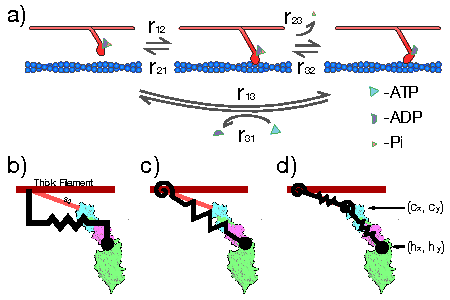
\includegraphics[width=3.2in]{../imgs/Figure1.pdf}
    \caption{
        \label{fig_xb_types}
        \textbf{Kinetic scheme and crossbridge types under investigation.} 
        The three state kinetic system is shown in subfigure A. 
        The three states represent (1) an unbound state, (2) a weakly bound state, and (3) a strongly bound state. 
        The binding rate ($r_{1,2}$), strong transition rate ($r_{2,3}$), and unbinding rate ($r_{3,1}$) are determined by the energy stored in the springs representing the crossbridge. 
        The reverse rates ($r_{2,1}$, $r_{3,2}$, and $r_{1,3}$) are functions of the forward transition rates.
        Subfigures B, C, and D show the crossbridge representations we examine, plotted against a myosin crystal structure for comparison (crystal structure image generated from \citet{Gourinath2003} with MacPyMol). 
        Subfigure B shows the single-spring crossbridge (1sXB) used heavily used in models since \protect\citep{Huxley1957}. 
        Subfigure C depicts the two-spring crossbridge (2sXB) which uses both a torsional/angular spring and a linear spring. 
        Subfigure D shows a four-spring crossbridge (4sXB) using two torsional and two linear springs, which we compare the single and dual spring crossbridges against. 
        % TODO : Take out the next two lines or make them useful.
        The locations of the distal torsional spring and tip of the 4sXB are denoted as $(c_x, c_y)$ and $(h_x, h_y)$ respectively. 
        The tip of the 2sXB is also denoted as $(c_x, c_y)$.
    }
    \end{center}
\end{figure}

\begin{figure}[htbp]
    \begin{center}
    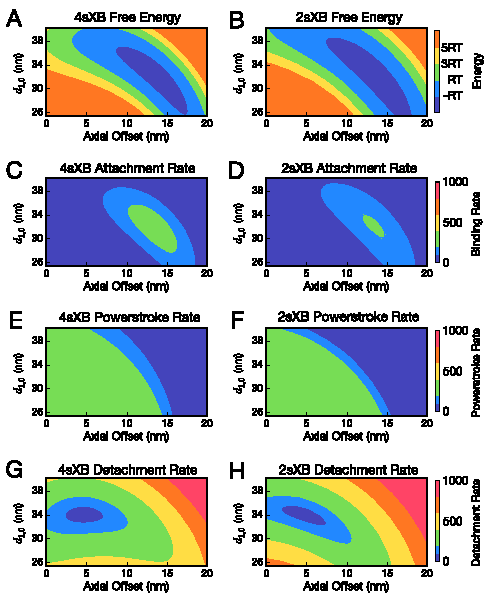
\includegraphics[width=3.2in]{../imgs/Figure2.pdf}
    \caption{
        \label{fig_kinetics_contours}
        \textbf{Energy and kinetics of the 4sXB and 2sXB systems at varying axial offsets and lattice spacings.} 
        Subfigures A through H show the properties of the 4sXB (subfigures A, C, E, and G) and the 2sXB (subfigures B, D, F, and H) as they change with binding site offset and $d_{1,0}$ lattice spacing.
        Binding site offset is the distance between the current axial location of the crossbridge's tip, $h_x$, and the location where the crossbridge attaches to the thick filament.
        Lattice spacing ($d_{1,0}$) is defined as in \citet{Millman1998}, with an offset to account for filament thicknesses so that the crossbridge exactly bridges the two filaments at a rest lattice spacing of 34 nm.
        Subfigure A depicts the free energy of the 4sXB at various lattice spacings (represented along the y-axis), with the head stretched to an axial offset from the thick filament attachment point (zero on the x-axis).
        Similarly, the free energy of the 2sXB is shown in subfigure B.
        The lowest energy myosin head locations in both A and B are shown as the darkest part of the plot and change in axial offset as lattice spacing changes.
        The subfigures C and D show $r_{1,2}$, the probability that the 4sXB and the 2sXB will transition from an unbound state to a bound state, and the dependence of this transition on both the axial offset of the open binding site from the myosin thick filament attachment site and the lattice spacing $d_{1,0}$ which is a function of the distance between the binding site and the thick filament attachment point of the myosin head. 
        Subfigure C depicts this probability for the 4sXB as a two dimensional contour with the same axes as in A while subfigure D depicts the transition probabilities for the two spring crossbridge.
        Subfigures E and F show $r_{2,3}$, the probability of transition from a weakly bound state to a strongly bound state, for the same crossbridges, with the same axes and scales as C and D show $r_{1,2}$.
        Subfigures G and H show $r_{3,1}$, the probability of unbinding from a strongly bound state, for the same crossbridges, with the same axes and scales as C and D show $r_{1,2}$.
        The reverse rates, $r_{2,1}$, $r_{3,2}$, and $r_{1,3}$ may be back-calculated from the forward rates.
    }
    \end{center}
\end{figure}

\begin{figure}[htbp]
    \begin{center}
    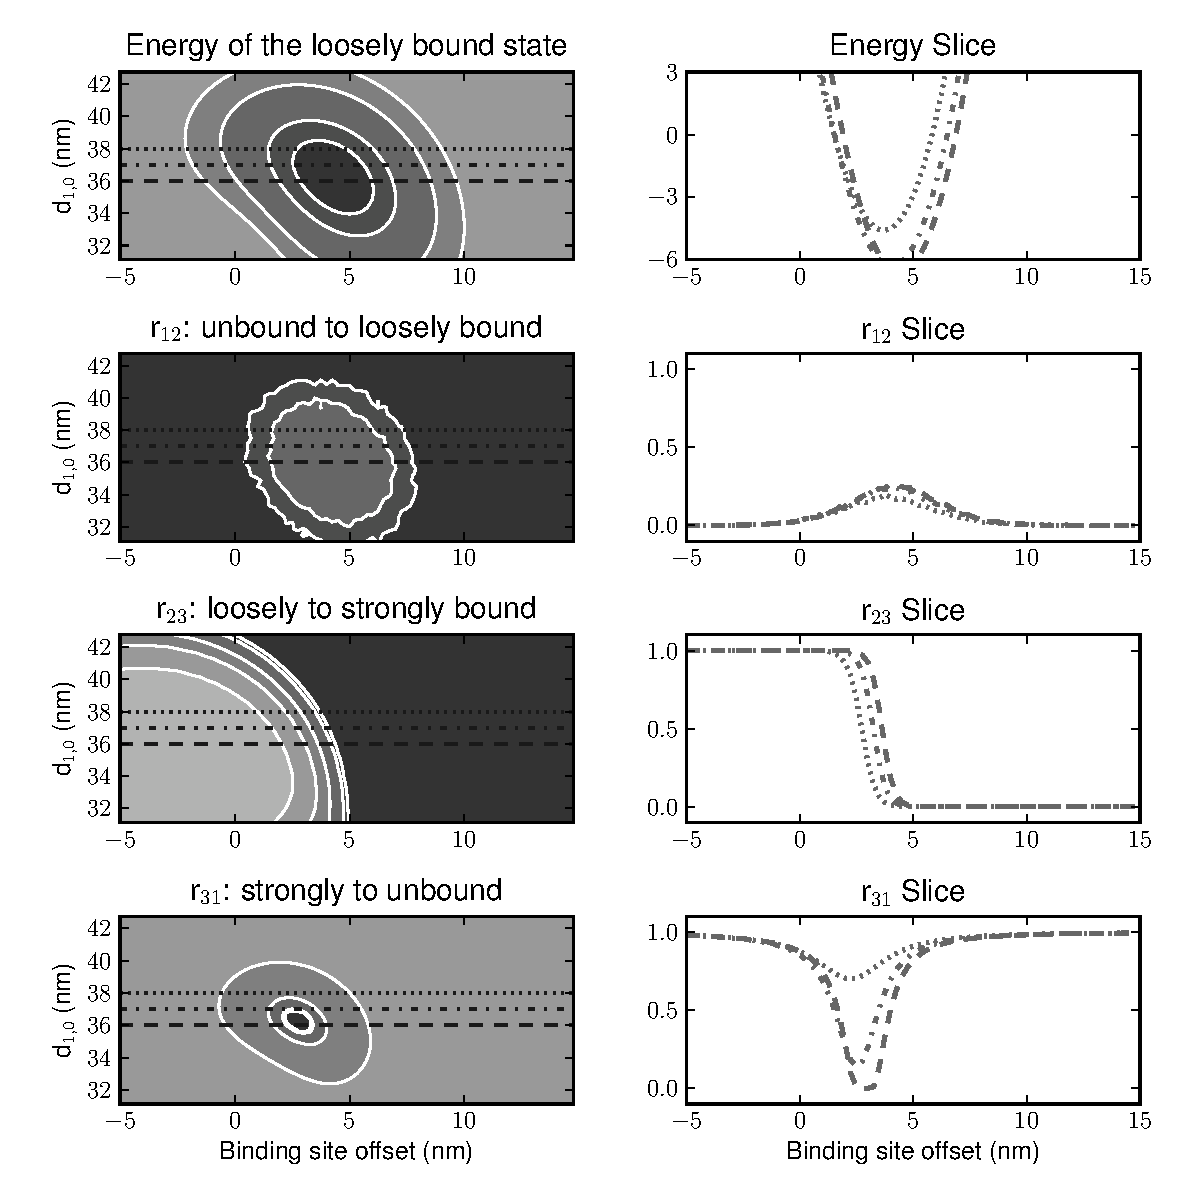
\includegraphics[width=3.2in]{../imgs/Figure3.pdf}
    \caption{
        \label{fig_kinetics_cuts}
        \textbf{Energy and kinetics of the 1sXB, 2sXB, and 4sXB at the resting lattice spacing.}
        Subfigures A through D show the energy and transition rates of the 1sXB (black), 2sXB (green), and 4sXB (red) at resting lattice spacing.
        The 1sXB values shown for comparison are derived from those of \citet{Daniel1998} and \citet{Tanner2007}, shifted axially so the resting location of the crossbridge head in each case is aligned with that of the 2sXB and 4sXB. 
        The free energy of the crossbridges in state two is shown in subfigure A, where the multi-spring crossbridges' shifts from a strictly parabolic trajectory is visible.
        The explicit thermal forcing of the multi-spring crossbridge heads in subfigure B results in binding probabilities that are more distributed than those of the single spring crossbridge.
        The rate of powerstrokes, in subfigure C, remains least changed between the single and the multi-spring crossbridge models.
        The energy-based kinetics of the multi-spring crossbridges are unable to fully replicate the biased detachment rate of the 1sXB in subfigure D. 
    }
    \end{center}
\end{figure}

\begin{figure}[htbp]
    \begin{center}
    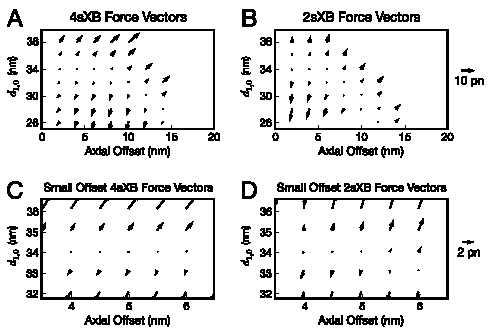
\includegraphics[width=3.2in]{../imgs/Figure4.pdf}
    \caption{
        \label{fig_forces}
        \textbf{Overview and detail of the forces exerted by the 2sXB and 4sXB.}
        Subfigures A through D show the forces exerted by the 4sXB and the 2sXB, with the shade of the vector arrows being determined by the chance of such a configuration occurring, a sum of the $r_{23}$ and the inverse of the $r_{31}$ transition probabilities. 
        Subfigures A and B show overviews of the forces exerted, respectively, by the 4sXB and the 2sXB over lattice spacings and axial offsets that vary as in Figure 2.
        The forces exerted by the two crossbridges have radial components which frequently equal or exceed their axial components.
        A more detailed view of the region surrounding the rest position of the crossbridges is shown in subfigures C and D, where the large radial components of the crossbridge forces, particularly for the 2sXB, is again evident.
        Subfigures E through H show, separated, the axial and radial components of the 4sXB and the 2sXB.
    }
    \end{center}
\end{figure}

% bibliography (fold)
% Bib style requires biophysj.bst be in the document directory
\clearpage
\bibliographystyle{biophysj}
\bibliography{JournalArticles,NotArticles}
% bibliography (end)

\end{document}
